% This is a LaTeX thesis template for Monash University.
% to be used with Rmarkdown
% This template was produced by Rob Hyndman
% Version: 6 September 2016

\documentclass{monashthesis}

%%%%%%%%%%%%%%%%%%%%%%%%%%%%%%%%%%%%%%%%%%%%%%%%%%%%%%%%%%%%%%%
% Add any LaTeX packages and other preamble here if required
%%%%%%%%%%%%%%%%%%%%%%%%%%%%%%%%%%%%%%%%%%%%%%%%%%%%%%%%%%%%%%%

\author{Xiefei Li}
\title{Revisiting the Forecast Combination Puzzle: An Empirical Study}
\studentid{30204232}
\studentemail{\href{mailto:xlii0145@student.monash.edu}{\nolinkurl{xlii0145@student.monash.edu}}}
\studentdetails{Supervisor: David T. Frazier}
\supervisoremail{\href{mailto:David.frazier@monash.edu}{\nolinkurl{David.frazier@monash.edu}}}
\def\degreetitle{Bachelor of Commerce (Honours)}
% Add subject and keywords below
\hypersetup{
     %pdfsubject={The Subject},
     %pdfkeywords={Some Keywords},
     pdfauthor={Xiefei Li},
     pdftitle={Revisiting the Forecast Combination Puzzle: An Empirical Study},
     pdfproducer={Bookdown with LaTeX}
}


\bibliography{thesisrefs}

\begin{document}

\pagenumbering{roman}

\titlepage

{\setstretch{1.2}\sf\tighttoc\doublespacing}

\clearpage\pagenumbering{arabic}\setcounter{page}{1}

\hypertarget{abstract}{%
\chapter*{Abstract}\label{abstract}}
\addcontentsline{toc}{chapter}{Abstract}

The abstract should outline the main approach and findings of the thesis and must not be more than 500 words.

Finish up afterwards.

\newpage

\hypertarget{acknowledgements}{%
\chapter*{Acknowledgements}\label{acknowledgements}}
\addcontentsline{toc}{chapter}{Acknowledgements}

I would like to thank my supervisor, my Honours coordinator, all the people who helped me throughout the year and myself.

\hypertarget{introduction}{%
\chapter{Introduction}\label{introduction}}

\hypertarget{research-objective}{%
\section{Research Objective}\label{research-objective}}

This thesis aims to investigate the determinants behind, and evidence for the forecast combination puzzle in various domains, and to empirically examine a general solution to the forecast combination puzzle. The combination puzzle refers to the well-known empirical finding that an equally weighted combination of forecasts generally outperforms more sophisticated combination schemes. This phenomenon is often found in the point forecast combinations but it is also the case in the density forecast combinations. Starting with time series data, this paper explores how the puzzle is affected by the fitness of models on the high volatile or the strong seasonal dataset. The empirical studies undertaken so far have focused more on pure time series settings, while there is little literature on the presence of the combination puzzle in the cross-sectional setting. A simulated study is conducted to study the puzzle in the two-model combination under a regression analysis. The performance of density combinations will be assessed via the log score function and mean squared forecast error is used to assess the point combinations for seasonal data. As an additional contribution, we will assess the veracity, and applicability, of a recently proposed solution to the forecast combination puzzle suggested in \textcite{ZMFP22} and \textcite{FZMP23}.

\hypertarget{literature-review-and-motivation}{%
\section{Literature Review and Motivation}\label{literature-review-and-motivation}}

The forecast accuracy is of critical concern for forecasters and decision makers. With the evidence of dramatic improvements in the forecast accuracy, forecast combinations have attracted wide attention and contributions in the literature, both theoretical and applied \autocite{C89,T06}. More importantly, this promising approach often has a robust performance for various types of series, which is borne out by numerous empirical results \autocite{GA11}. \textcite{MACF82} carefully examined the forecast accuracy with a considerable amount of time series, and reported that forecast combinations perform better than individual models. Later, \textcite{SW98} claimed that the best-performing single method can be further improved by incorporating other forecasts, based on empirical comparisons of different forecasting methods. Despite of the point forecasting, researchers also devote efforts on probabilistic forecasting with more information about uncertainties and continue to find that optimal density forecast combination outperforms individual forecasts \autocites[e.g.,][]{HM07,GA11}.

Forecast combinations refer to the idea of combining multiple forecasts generated from possible models, which was originally proposed in the seminal work of \textcite{BG69}. The forecast combination methods, in general, involve producing forecasts from constituent models, and then combining them based on a rule or weighting scheme. Each scheme has different selection criteria for the ``best'' forecast combination and the corresponding weight value assigned to each model. This process can sometimes capture more meaningful characteristics of the true data generating process than using a single model, and allow us to combine the best features of different models within a single framework. Researchers have examined a variety of combination methods for both point and density forecasts over the past 50 years, see \textcite{WHLK22} for a modern literature review.

In most time series setting under which forecast combinations are employed, a striking empirical phenomenon is often observed, coined by \textcite{SW04}, as the ``forecast combination puzzle''. The puzzle is encapsulated by the fact that ``theoretically sophisticated weighting schemes should provide more benefits than the simple average from forecast combination, while empirically the simple average has been continuously found to dominate more complicated approaches to combining forecasts'' \autocite{WHLK22}. In other words, complex weighting schemes are designed to improve the accuracy, so these refined forecast combinations should perform better in theory. However, the mean of the contemporaneous forecasts appears to be more robust in practice than weighted forecasts combined through complicated schemes. This finding has been reaffirmed by extensive literature reviews and papers \autocites[e.g.,][]{C89,SW98,SW04,SW09,MSA18,MSA20}, and simple averaging naturally becomes a benchmark.

There are two possible explanations for the puzzle in the literature. One concentrates on the estimation uncertainty in combination weight \autocite{SW98,SW04,SW09}. Complicated weighting schemes introduce variability and uncertainty when estimating parameters, whereas the simple averaging does not require any estimation. The higher average loss and instability in the study of \textcite{SW04} were a strong evidence for the inferior performance of sophisticated weighting schemes. On the other hand, \textcite{E11} and \textcite{CMVW16} explore the trade-off between bias and variance in the Mean Squared Forecast Error (MSFE). \textcite{CMVW16} demonstrated the presence of bias and inefficiency when weights estimation is required, in comparison with the fixed-weights such as the equal weights. They further proved that equally weighted combination is unbiased and its variance has only one component, resulting in a smaller mean squared error than a biased combination. However, this is applicable and specific to the MSFE scheme.

While various explanations for the forecast combination puzzle have been suggested over the years (see the above references), a general solution to the puzzle has so far proved elusive. Recently, \textcite{ZMFP22} and \textcite{FZMP23} proposed a new explanation for the puzzle in a general way by investigating the sampling variability of the forecasts induced via estimation of the constituent model forecasts (i.e., the models used to produce the forecasts). They illustrated that, asymptotically, the bias and variability mainly come from the estimation of the models used to produce the constituent model forecasts. The common way of producing forecast combinations keeps the model estimation uncertainty fixed during the weight estimation process, which is one reason of having the puzzle. If constituent models and weights can be estimated jointly, if feasible, the puzzle can be eliminated suggested by \textcite{FZMP23}. Under this approach, the sophisticated weighting schemes should (asymptotically) be superior.

Following the research direction of \textcite{BS16}, we are looking for a relationship between model fitting and the presence of the puzzle in the case of two-model combination. We speculate that the puzzle is only revealed when both constituent models are correctly specified and fit the data well. If one of them fails to capture the data patterns, the forecast combination will give more weight to the better model. Even if both models are misspecified, the complicated weighing scheme will try to reduce the uncertainty of the worse model as much as possible. Table \ref{tab:1} visually summarizes the conjectures.

\begin{table}[ht]
\centering
\begin{tabular}{cccc}
                       &      & \multicolumn{2}{l}{$M_2$} \\
                       &      & Good       & Bad       \\
\multirow{2}{*}{$M_1$} & Good & $\surd$    & $\times$ \\
                       & Bad  & $\times$   & $\times$
\end{tabular}
\caption{The first row and the first column refer to two constituent models in a combination, $M_1$ and $M_2$. Good indicates the model is correctly specified and fits the data well, whereas Bad denotes the model is misspecified and fails capture the important features of the data. The ``$\surd$`` implies the presense of the forecast combination puzzle, while ``$\times$`` means no forecast combination puzzle.}
\label{tab:1}
\end{table}

Even though there is a widespread literature among different pure time series settings, no attention appears to have been given to the cross-sectional setting. We investigate the forecasting performance of cross-sectional data and misspecified models via a simulation study. At a glance, the presence of the puzzle is determined by at least 3 elements in the two-model pools, which are the sample size, the true value of parameters except the intercept, and the variances of regressors.

The goal of this thesis is manifolds: first, to substantiate the presence of the combination puzzle in the usual time series in which it has been found; second, to examine the relationship between the puzzle and the model specification; third, to search for empirical evidence of the combination puzzle in cross-sectional settings; fourth, to test the empirical veracity of the theoretical solution to the puzzle found in \textcite{FZMP23}, both within, and outside of, the standard time series setting where the puzzle is often observed.

\hypertarget{method}{%
\chapter{Methodology}\label{method}}

The first goal of this paper is to construct linear density forecast combinations with parametric models. The results are anticipated to reveal that forecast combinations can deliver improved accuracy over single models, but are not necessarily superior to forecasts obtained from the equally weighted combination.

The next goal is to estimate the unknown parameters of the constituent models and the weight in a single step, and to compare the accuracy of forecasts based on these combinations against the usual combinations process, as well as the equally weighted combination. To measure differences between these forecasts, we will eventually employ forecast accuracy tests, of the type derived in \textcite{W96}, which measure out-of-sample differences between forecasts.

In the literature, there are several definitions of combinations. We focus on the combination of forecasts from independent models for a given dataset, which is commonly performed in two stages:

\begin{enumerate}
\def\labelenumi{\arabic{enumi}.}
\item
  producing separate point or probabilistic forecasts for the next time point using observed data and constituent models, and
\item
  combining forecasts based on one of the accuracy criteria.
\end{enumerate}

Specifically, considering the combination of two individual forecasts allows us to delve into interesting and unexplained findings through fast data manipulation \autocite{BS16}.

Before explaining further details, the following notation will be used throughout the paper. A vector time series \(\textbf{y}_t\) with a total of \(T\) observations will be divided proportionally into two parts, an in-sample period \(R\) and an out-of-sample period \(P\). The realization of a target variable \(y\) at time \(t\) is denoted as \(y_{t}\). Its future values after the in-sample period is denoted as \(y_{\small{R+h}}\), where \(h\) is the forecast horizon and \(h>0\). The information set at time t, \(\mathcal{F}_t\), is comprised of all observed (and known) realizations of \(y\) up to time t, i.e., \(\mathcal{F}_t = \{y_1, y_2, .., y_t\}\).

The choice and specification of constituent models are determined by the features of the in-sample data. For each model, the error term is assumed to be independent and normally distributed so that the Maximum Likelihood Estimation (MLE) method can be applied to generate the estimators of unknown parameters. Given the log likelihood function of in-sample period for each model, the corresponding estimates are obtained when they maximize that function and then held fixed for the following procedures. The optimal combination is then constructed with the estimated weight of each model that delivers the best accuracy.

A parametric model \(M\) determines the conditional probability density for \(\textbf{y}_t\), denoted by \(f(y_t|\mathcal{F}_{t-1}, \theta_M, M)\), given unknown parameters \(\theta_M\) and all the past information \(\mathcal{F}_{t-1}\). The choice and specification of constituent models vary by the features of the in-sample data. For each model, the error term is assumed to be independent and normally distributed so that the Maximum Likelihood Estimation (MLE) method can be applied to generate the estimators of unknown parameters, i.e., \(\hat\theta_M = \underset{\theta_M}{\arg\max} \sum^R_{t=1} log f(y_t|\mathcal{F}_{t-1}, M)\). Given the log likelihood function of in-sample period for each model, the corresponding estimates are obtained when they maximize that function and then held fixed for the following procedures.

One thing to clarify is that we do not consider the properties of estimators, so model misspecification will not ruin the results. CHECK!!!!

\hypertarget{density-combinations}{%
\section{Density combinations}\label{density-combinations}}

\hypertarget{linear-pooling}{%
\subsection{Linear pooling}\label{linear-pooling}}

Consider the case of only two competing probability densities, undoubtedly, densities can be combined in many ways; see Section 3 of \textcite{WHLK22} for many popular means of probabilistic combination. One of the commonly used approaches is the ``linear opinion pool'': aggregate constituent weighted densities in a linear form \autocites[e.g.,][]{BG69,HM07,GA11}. For the \texttt{two-model} pools, constituent densities \(f_1(y_t)\) and \(f_2(y_t)\) are combined as follows:

\begin{equation}
\label{eqn:LC1}
f(y_t) = w \ f_1(y_t | \mathcal{F}_{t-1}, \hat\theta_{M1}, M_1) + (1-w) f_2(y_t | \mathcal{F}_{t-1}, \hat\theta_{M2}, M_2)
\end{equation}

where \(w\) is the non-negative weight allocated to the probability density derived from the first model. Through this construction, the sum of two weights is implied to be 1, which is a necessary and sufficient condition for \(f(y_t)\) to be a proper density function \autocite{GA11}. In addition to point forecasts, the use of density forecasts can offer forecasters or decision markers a more comprehensive view of the target variable (see section 2.6.1. of \textcite{FTP22} for related contributions).

\hypertarget{log-socring-rules}{%
\subsection{Log socring rules}\label{log-socring-rules}}

Following the literature on density evaluation, our initial analysis will focus on using the log score function to measure the accuracy of our density forecasts; see, e.g., \textcite{GA11} for a discussion on log score and its use in density forecasting. For each individual model \(M\), the log score over the sample \(t = 1, \dots, T\) is:

\begin{equation}
\label{eqn:LS1}
LS = \sum^T_{t=1} log \ f(y_t| \mathcal{F}_{t-1}, \hat\theta_M, M).
\end{equation}

The ``optimal'' linear combination is identified to produce the most accurate forecasts when the set of weights maximizes the log score function of two densities over the in-sample \(t = 1, 2, \dots, R\).

\begin{equation}
\label{eqn:LS2}
\hat{w}_{\text{opt}} = \underset{w}{\arg\max} \sum^R_{t=1} log \Big[ w \ f_1(y_t| \mathcal{F}_{t-1}, \hat\theta_{M1}, M_1) + (1-w) \ f_2(y_t| \mathcal{F}_{t-1}, \hat\theta_{M2}, M_2)\Big]
\end{equation}

Thus, the log predictive score over the forecast horizon \(h = 1, 2, \dots, P\) (i.e., the out-of-sample period) is:

\begin{equation}
\label{eqn:LS3}
LPS = \sum^T_{t = R+1} log \Big[ \hat{w}_{\text{opt}} \ f_1(y_t| \mathcal{F}_{t-1}, \hat\theta_{M1}, M_1) + (1- \hat{w}_{\text{opt}}) \ f_2(y_t| \mathcal{F}_{t-1}, \hat\theta_{M2}, M_2)\Big].
\end{equation}

\hypertarget{point-combinations}{%
\section{Point combinations}\label{point-combinations}}

For time series with seasonal patterns, we follow \textcite{BG69} and \textcite{SW09}, and consider the combination of pairs of point forecasts for the ease of calculation. Same as \textcite{SW09}, the mean squared forecast error (MSFE) is adopted to measure the point forecast accuracy.

\hypertarget{linear-combination}{%
\subsection{Linear combination}\label{linear-combination}}

Similar to the density case, point predictions from two models, \(\hat y_{1t}\) and \(\hat y_{2t}\), are aggregated linearly:

\begin{equation}
\label{eqn:PC1}
\hat y_t = w \ \hat y_{1t} + (1-w) \ \hat y_{2t}
\end{equation}

where \(w\) is the non-negative weight allocated to the point prediction generated from the first model.

\hypertarget{mean-squared-forecast-error-msfe}{%
\subsection{Mean squared forecast error (MSFE)}\label{mean-squared-forecast-error-msfe}}

The MSFE is defined as

\begin{equation}
\label{eqn:MSFE1}
\frac{1}{P} \sum^T_{t=R+1} (y_t - \hat y_t)^2.
\end{equation}

The ``optimal'' set of weights satisfies that it minimizes the MSFE among all other possible sets.

\hypertarget{empirical-results}{%
\chapter{Empirical Results}\label{empirical-results}}

\hypertarget{pure-time-series-setting-sp-500}{%
\section{Pure time series setting (S\&P 500)}\label{pure-time-series-setting-sp-500}}

Reconsidering the example in Section 3 of \textcite{GA11}, the data we use is the daily Standard and Poor's (S\&P) 500 index from February 11, 2013 to February 10, 2023 (10 years in total), retrieved from the \textcite{SP500}. The S\&P500 index dataset has a total of 2519 (\(T\)) observations and is partitioned into two periods with a rough proportion. The in-sample period contains the first 60\% of the data (\(R = 1511\)), which is used to estimate all unknown parameters, including the optimal weight. The remaining 40\% (\(P = 1008\)) becomes the out-of-sample period to evaluate the forecast performance.

We will investigate the presence of the forecast combination puzzle when using correctly-specified models or mis-specified models to fit the data. Constituent models are based on common classes of models: autoregressive integrated moving average (ARIMA), exponential smoothing (ETS), and linear regression model with ARIMA errors. Detailed model specifications for each case will be clarified in the corresponding section.

We choose \(j=1,\cdots,M\), with \(M=3\) prediction models to study the performance of density predictions across sets of \texttt{two-model} pools. Each of the \(j\) predictive model has a conditional Gaussian density, which takes the form \(f^{(j)}(y)=f_j(y_t|\mathcal{F}_{t-1})=N\{y_t; \mu_j, \sigma^2_j\}\), where \(N\{x; \mu, \sigma^2\}\) denotes the normal probability density function evaluated at value \(x\) with mean \(\mu\) and variance \(\sigma^2\). The notation \(\mathcal{F}_{t-1}\) denotes all information available at time \(t-1\), and we assume that the conditional mean and variance of the models are, up to unknown parameters, known at time \(t-1\).

\hypertarget{nonstationary-time-series}{%
\subsection{Nonstationary time series}\label{nonstationary-time-series}}

To reduce the level of variability, we take a natural logarithm of the S\&P 500 index \(y_t\) and fit the data directly without removing its stochastic trend with three candidate models.

\begin{enumerate}
\def\labelenumi{\arabic{enumi}.}
\item
  ARIMA(1,1,1) model with an intercept of the natural logarithm of S\&P 500 index.
  \begin{equation*}
  log(y_t) = c + log(y_{t-1}) + \phi_1\big[log(y_{t-1})-log(y_{t-2})\big] + \epsilon_t + \theta_1\epsilon_{t-1}
  \end{equation*}
\item
  ETS(M,N,N) model of the natural logarithm of S\&P 500 index.
  \begin{align*}
  log(y_t) &= \ell_{t-1} (1+\epsilon_t) \\
  \ell_t &= \ell_{t-1} (1+\alpha \epsilon_t) \\
  \end{align*}
\item
  A classical linear regression model of the natural logarithm of the S\&P 500 index and ARIMA(1,0,0) errors.
  \begin{align*}
  log(y_t) &= \beta_0 + \beta_1 t + u_t \\
  u_t &= \phi_1 u_{t-1} + \epsilon_t
  \end{align*}
\end{enumerate}

The error term, \(\epsilon_t\), in each model is assumed to be independent and normally distributed with a zero mean and a constant variance.

There are three sets of two-model combinations in total. Consider the weight \(w\) takes a value from 0 to 1 and changes by 0.01 every time. The log score, as a function of weight, is generated to search for the optimal weight over the in-sample \(R\) period (refer to the top row of Figure \ref{fig:nonstat}). According to equation \ref{eqn:LS2}, the estimated optimal weight corresponds to the maximum point of the curve. Then we can calculate the log predictive score of the optimal combination for the out-of-sample period based on equation \ref{eqn:LS3}.

\begin{table}[ht]
  \centering
  \caption{Log predictive score of density forecasts combination under two-model pools of S\&P 500}
    \begin{tabular}{lccc}
    \toprule
                 & ARIMA(1,1,1)       & ETS(M,N,N)         & LR \\
    \midrule
    ARIMA(1,1,1) & \textit{2345.9262} & 2441.7832          & 2362.7701 \\
    ETS(M,N,N)   & 0.65               & \textit{2442.2965} & 2423.2140 \\
    LR           & 0.41               & 0.21               & \textit{2338.6005} \\
    \bottomrule
    \multicolumn{4}{l}{\footnotesize The diagonal entries contains individual log predictive score calculated over the out-of-sample period with $P$ observations.}\\
    \multicolumn{4}{l}{\footnotesize The log predictive scores of optimal combinations over the out-of-sample period are located above the diagonal.}\\
    \multicolumn{4}{l}{\footnotesize Entries below diagonal show the estimated optimal weight of the model in that column in the two-model pool.}\\
    \end{tabular}
  \label{tab:2}
\end{table}

\begin{figure}[ht]
\centering
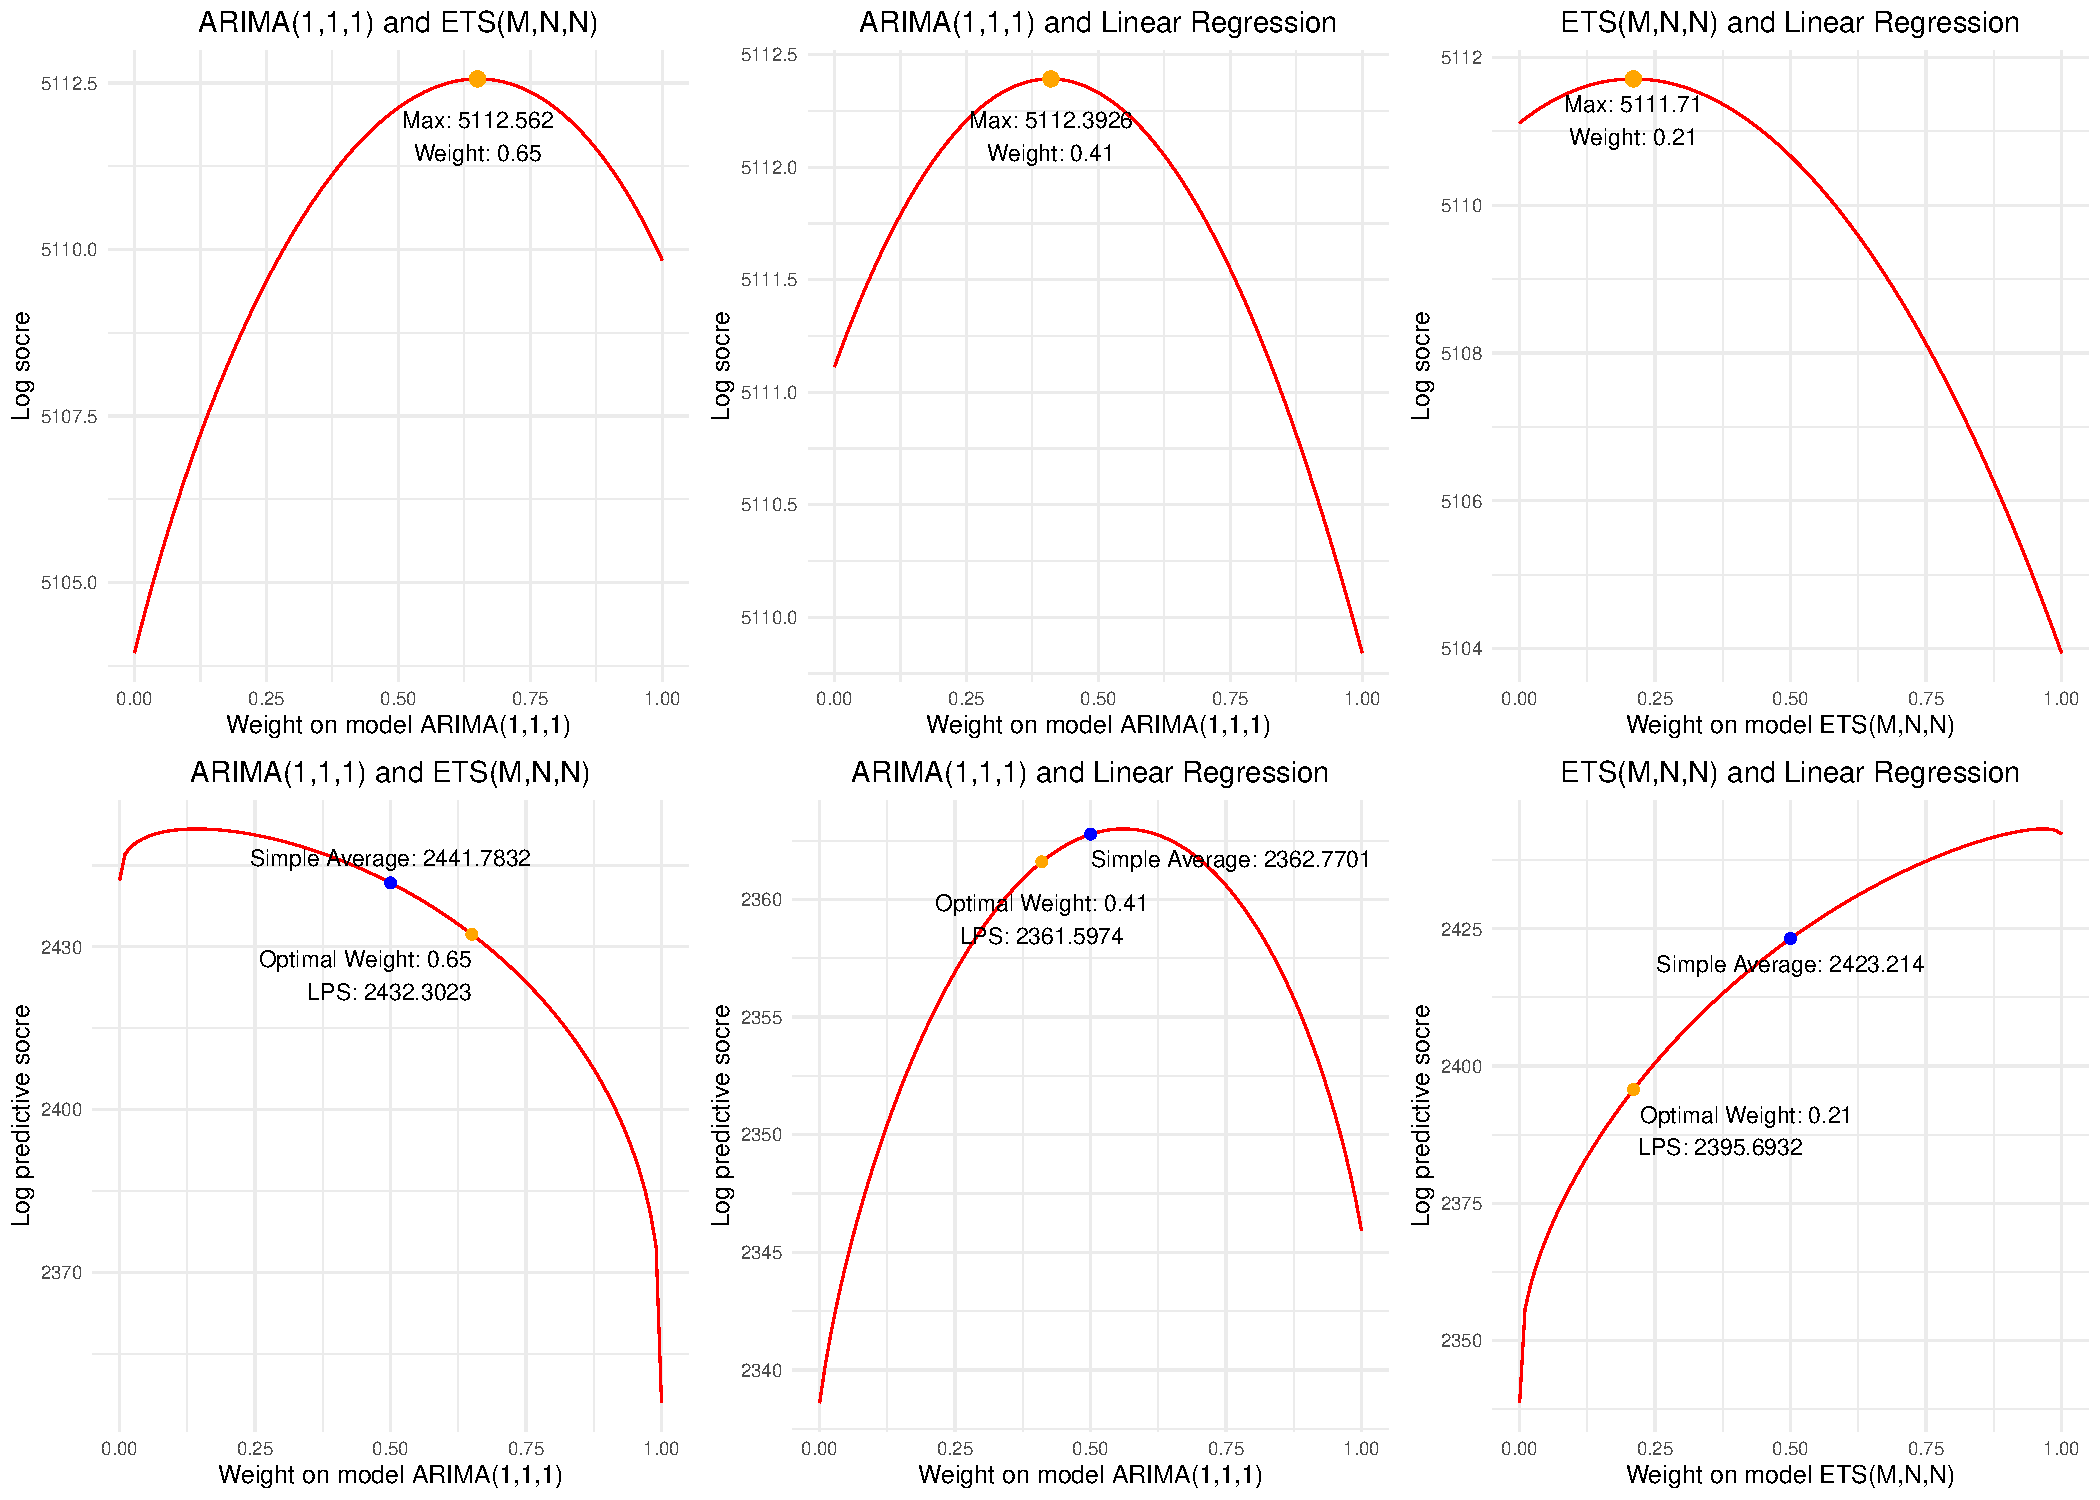
\includegraphics[scale=0.4]{figures/SP500_nonstationary.pdf}
\caption{Log predictive score in two-model pools over the in-sample (top) and out-of-sample (bottom) period of density combinations. Constituent prediction models described in the title. The x-axis represents the weight assigned on the former model of the combination and the y-axis indicates the log predictive score. The orange dot represents the optimal set of weights and the corresponding log predictive score in each case, while the blue dot indicates the forecast performance of the simple averaging method. The green dot, as a reference, refers to the maximum point of the out-of-sample curve.}
\label{fig:nonstat}
\end{figure}

Figure \ref{fig:nonstat} suggests that the forecast combination puzzle is only evident in the second predictive density combination (ARIMA(1,1,1) and Linear Regression). In the middle column, the log predictive score of the optimal combination, 2361.5974, is very close to that of the simple average combination, 2362.7701. However, the other two combinations do not reveal the puzzle. Besides, the simple average performs superior than the optimal combination in both cases.

\begin{figure}[ht]
\centering
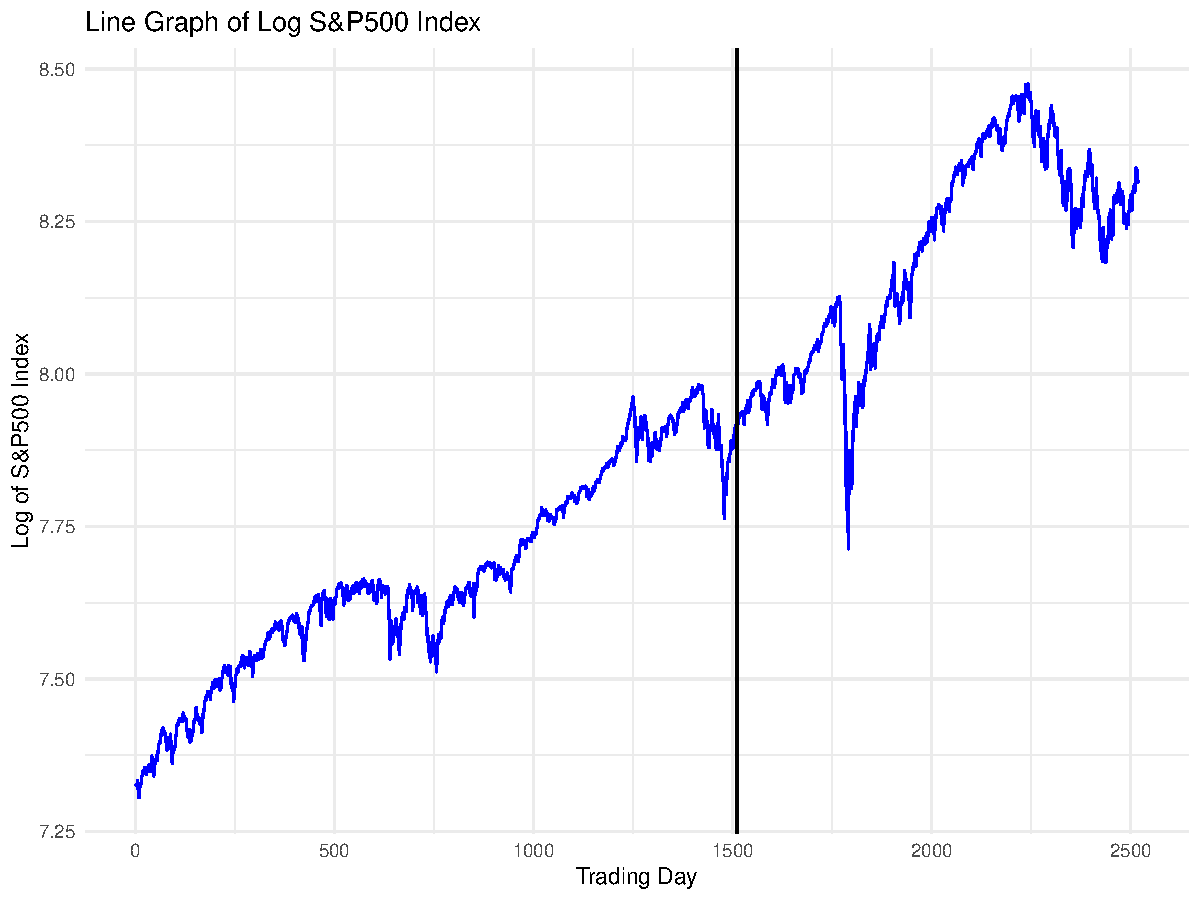
\includegraphics[scale=0.4]{figures/log_linegraph.pdf}
\caption{The black vertical line separates the traning set and the evaluation set. The training set is on the left and the evaluation set is on the right.}
\label{fig:llg}
\end{figure}

WHICH ONE???

ETS too bad?
One possible explanation could be that the ETS model badly fits the training set but forecasts well for the evaluation set in both cases. Given this data split, the optimal weight set gives less weight on the ETS model, leading to a low log predictive score for the optimal predictive density combination, compared with the simple average. This phenomenon implies that the optimal weight set could not be fixed but a varying variable when one of the constituent models does not fit well with the data. We conjecture that there is a relationship between the forecast combination puzzle and the fitness of constituent models.

ARIMA \& LR too good?

Since we are modelling the log of S\&P500, its trending behavior and structural breaks are dominant and need to be taken care of when fitting the model. That means a good model should capture the trend, deal with the structural breaks and incorporate all important features of this nonstationary data.

One possible explanation could be that the ARIMA model and the linear regression model fit the training set too well to take any future changes into consideration. It is also unanticipated to incorporate the large structural break and the changing slopes of the trend in the evaluation set as shown in Figure \ref{ig:llg}. Thus, their density forecast combinations end up with lower log predictive scores, compared with the simple average.

\hypertarget{stationary-time-series}{%
\subsection{Stationary time series}\label{stationary-time-series}}

Continuing with the same dataset, we now fit the stationary series by taking a first difference of the log of S\&P500. A series is said to be stationary when it has constant mean and variance, and its covariance depends on the time interval only. In other words, the entire series should have a roughly consistent pattern. Then, the training set and the evaluation set will not have completely different behaviors that highly influence the goodness-of-fit of models.

Consider two candidate models: a Gaussian ARMA(1,1) model and a classical linear regression model with ARMA(1,1) errors. Figure \ref{fig:stat} shows that two consitutent models have a very similar in-sample accuracy and the puzzle is obvious in the forecast combination. As expected, since both models fit the data well, the simply averaged point forecast performs almost the same as the optimal combined point forecast, indicating the presence of the forecast combination puzzle.

\begin{figure}[ht]
\centering
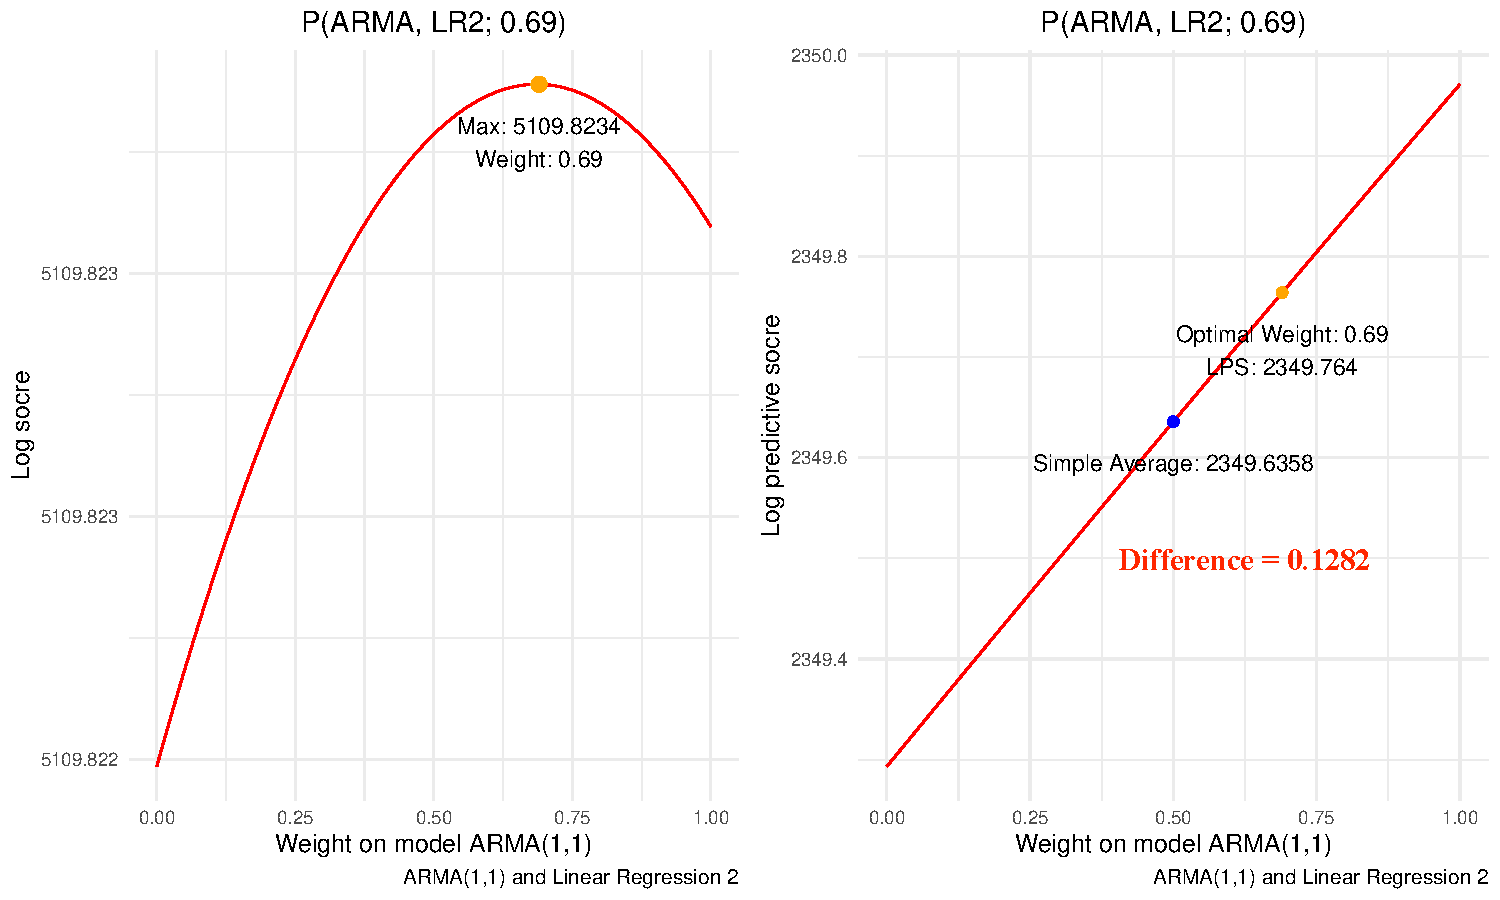
\includegraphics[scale=0.5]{figures/SP500_stationary.pdf}
\caption{Log predictive score in two-model pools over the in-sample (left) and out-of-sample (right) period of density combinations. The x-axis represents the weight assigned on the ARMA(1,1) model and the y-axis indicates the log predictive score. The meanings of colored dots remain the same}
\label{fig:stat}
\end{figure}

\hypertarget{pure-time-series-with-seasonality}{%
\section{Pure time series with seasonality}\label{pure-time-series-with-seasonality}}

With the purpose of corroborating above conjectures, we experiment with a quarterly dataset to observe the relationship between the puzzle and the specification of models. To make our life easier, we produce point forecasts and evaluate point combinations with Mean Squared Forecast Error.

The data considered is the quarterly total number of unemployed individuals (in thousands) from 1985 Q1 to 2023 Q1, retrieved from the Australia Bureau of Statistics \autocite{ABS}.

It has a total of 2519 (\(T\)) observations and is partitioned into two periods with a rough proportion. The in-sample period contains the first 60\% of the data (\(R = 1511\)), which is used to estimate all unknown parameters, including the optimal weight. The remaining 40\% (\(P = 1008\)) becomes the out-of-sample period to evaluate the forecast performance.

We will investigate the presence of the forecast combination puzzle when using both mis-specified and correctly-specified models to fit the data.

There are two combined point forecasts whose MSFEs are calculated over the last P observations

\hypertarget{misspecified-models}{%
\subsection{Misspecified models}\label{misspecified-models}}

With the purpose of examining the case when using two badly fit models, we experiment with seasonal dataset to observe the relationship between the puzzle and the specification of models.

\begin{figure}[ht]
\centering
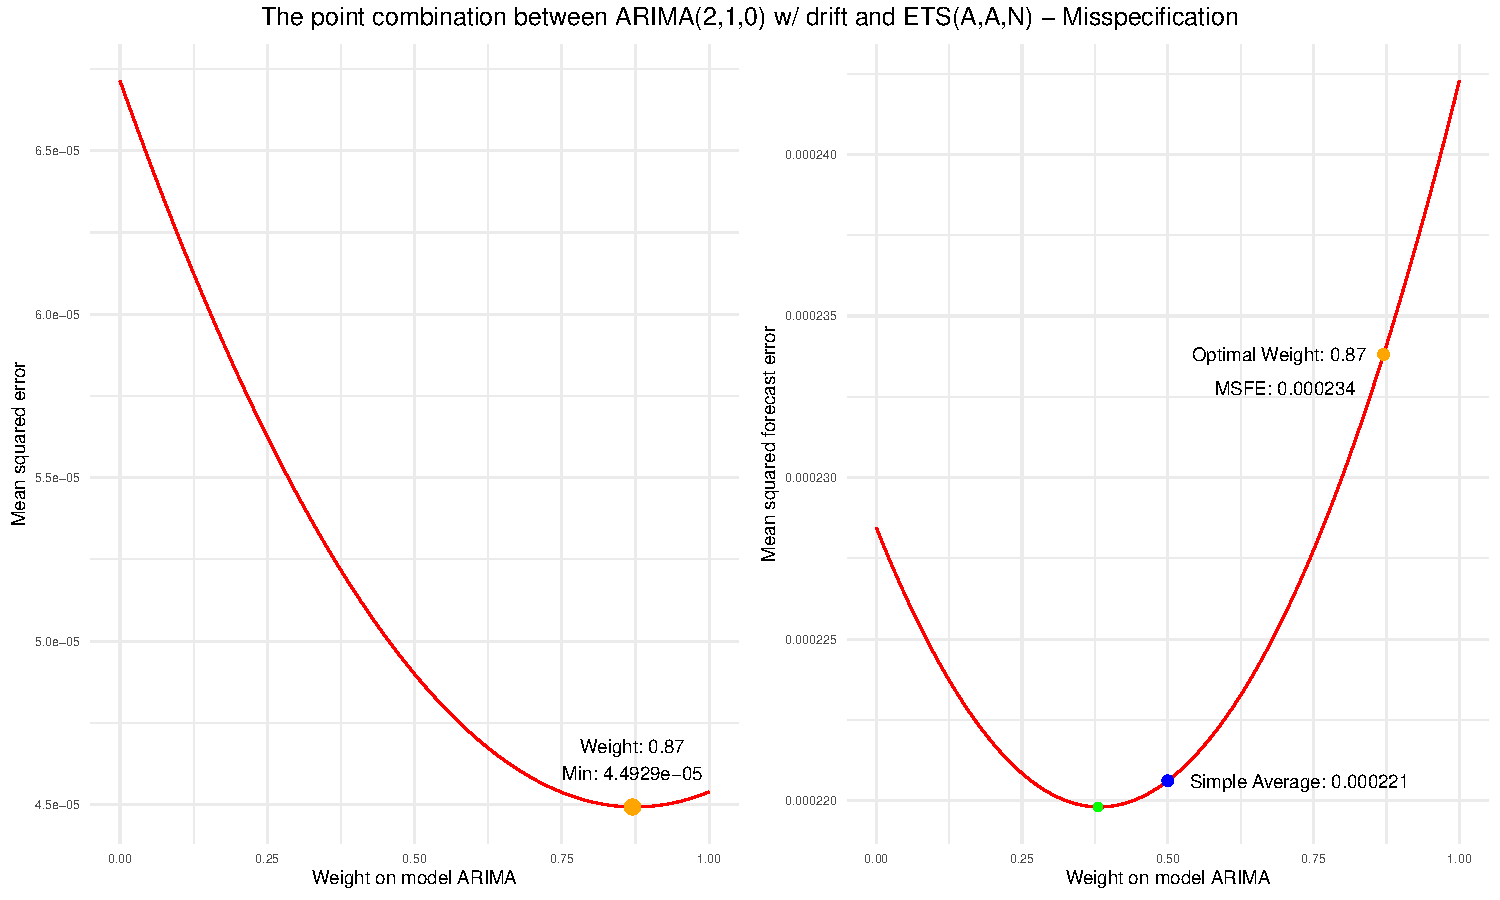
\includegraphics[scale=0.5]{figures/EMPL_misspecified.pdf}
\caption{}
\label{fig:sdm}
\end{figure}

\hypertarget{correctly-specified-models}{%
\subsection{Correctly specified models}\label{correctly-specified-models}}

\begin{figure}[ht]
\centering
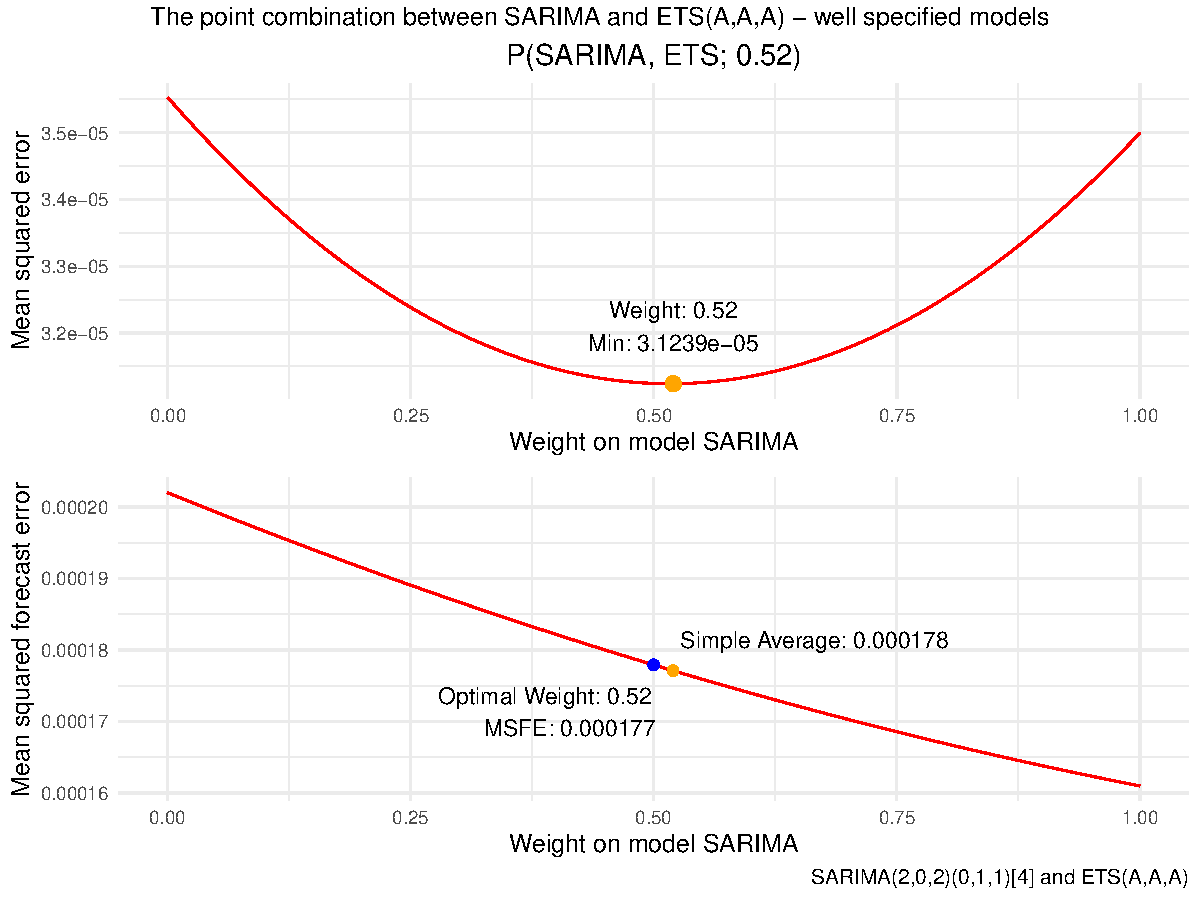
\includegraphics[scale=0.5]{figures/EMPL_correct.pdf}
\caption{}
\label{fig:sdc}
\end{figure}

\hypertarget{simulation-results}{%
\chapter{Simulation Results}\label{simulation-results}}

\hypertarget{pure-cross-sectional-setting}{%
\section{Pure cross-sectional setting}\label{pure-cross-sectional-setting}}

Given that the forecast combination can greatly improve the forecast accuracy, this idea of model combination can also be applied to the cross-sectional setting. Rather than forecasting future value, cross-sectional data often helps to better understand the individual behavior and decision-making with changing attributes.

A simulated cross-sectional dataset is designed to study how related elements in the linear regression model affect the presence of the puzzle, as well as the performance of density combinations. In line with previous notations but under the cross-sectional setting, the subscript \texttt{t} will change to \texttt{i} to represent each individual observation.

CHECK MOTIVATION!!!!

\hypertarget{experimental-design}{%
\subsection{Experimental design}\label{experimental-design}}

The true data-generating process (DGP) is assumed to be a classic linear regression model with only two exogenous and correlated regressors, which satisfies all classical assumptions:

\begin{equation}
\label{eqn:DGP}
y_i = \beta_0 + \beta_1 x_{1i} + \beta_2 x_{2i} + e_i, \ \ e_i \stackrel{i.i.d}{\sim} N(\mu_e,\sigma^2_e) \\
\end{equation}

where \(i\) represents each observation.

The initial set-up has 15000 (N) artificial cross-sectional observations generated from \ref{eqn:DGP} with \(E[x_{1i}] = E[x_{2i}] = 0\), \(Var(x_{1i}) = Var(x_{2i}) = 1\), \(Cov(x_{1i}, x_{2i}) = 0.7\), \(\pmb{\beta} = (\beta_0, \beta_1, \beta_2)' = (1,2,2)'\), \(\mu_e = 5\) and \(\sigma^2_e=10\).

Following the methodology in Section \ref{method}, the data will be divided into an in-sample period (roughly 60\%) for estimation and an out-of-sample period for accuracy evaluation. We propose two mis-specified models to generate density forecasts with each only contains one of the regressors. Assume Model 1 includes only \(x_{1i}\) as the regressor and the other model, Model 2, includes only \(x_{2i}\) as the regressor. The density forecast combinations will follow the construction of \texttt{two-model} pools and be evaluated by the log score functions.

\begin{itemize}
\item
  Sample size is \(N=15000\)
\item
  \(E[x_{1i}] = E[x_{2i}] = 0\)
\item
  \(Var(x_{1i}) = Var(x_{2i}) = 1\)
\item
  \(Cov(x_{1i}, x_{2i}) = 0.7\)
\item
  The true value of \(\pmb{\beta} = (\beta_0, \beta_1, \beta_2)' = (1,2,2)'\)
\item
  \(\mu_e = 5\) and \(\sigma^2_e=10\)
\end{itemize}

\begin{figure}[ht]
\centering
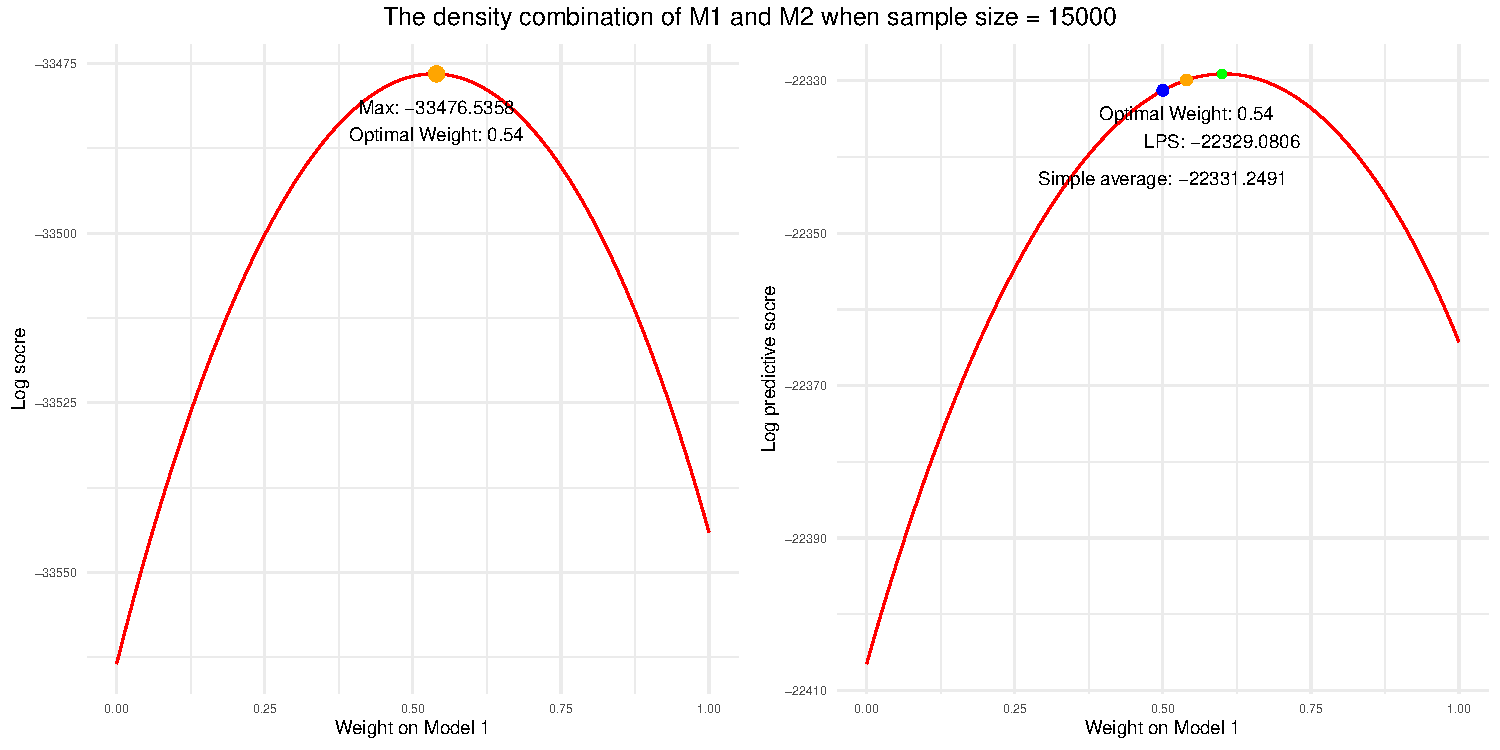
\includegraphics[scale=0.6]{figures/Sample_Size_15000.pdf}
\caption{Two curves refer to the in-sample (left) and out-of-sample (right) performance of density combinations with artificial cross-sectional data under the initial set-up. The x-axis represents the weight assigned on Model 1 and the y-axis indicates the log score for each density combination. The orange dot represents the optimal set of weights and the corresponding log predictive score in each case, while the blue dot indicates the forecast performance of the simple averaging method. The green dot, as a reference, refers to the maximum point of the out-of-sample curve.}
\label{fig:ss15000}
\end{figure}

Figure \ref{fig:ss15000} clearly reflects that when the sample size is large enough, the simple average of predicted densities, indicated by the blue dot, can retain the forecast accuracy with a small difference in the log predictive score, compared with the optimal combination indicated by the orange dot. This is an evidence of facing forecast combination puzzle. Given the puzzle, we can change the true value of relevant elements one at a time while holding all others constant, and then summarize the conditions under which the puzzle is likely to be evident.

\begin{itemize}
\tightlist
\item
  \bf{Sample Size}
\end{itemize}

\begin{figure}[ht]
\centering
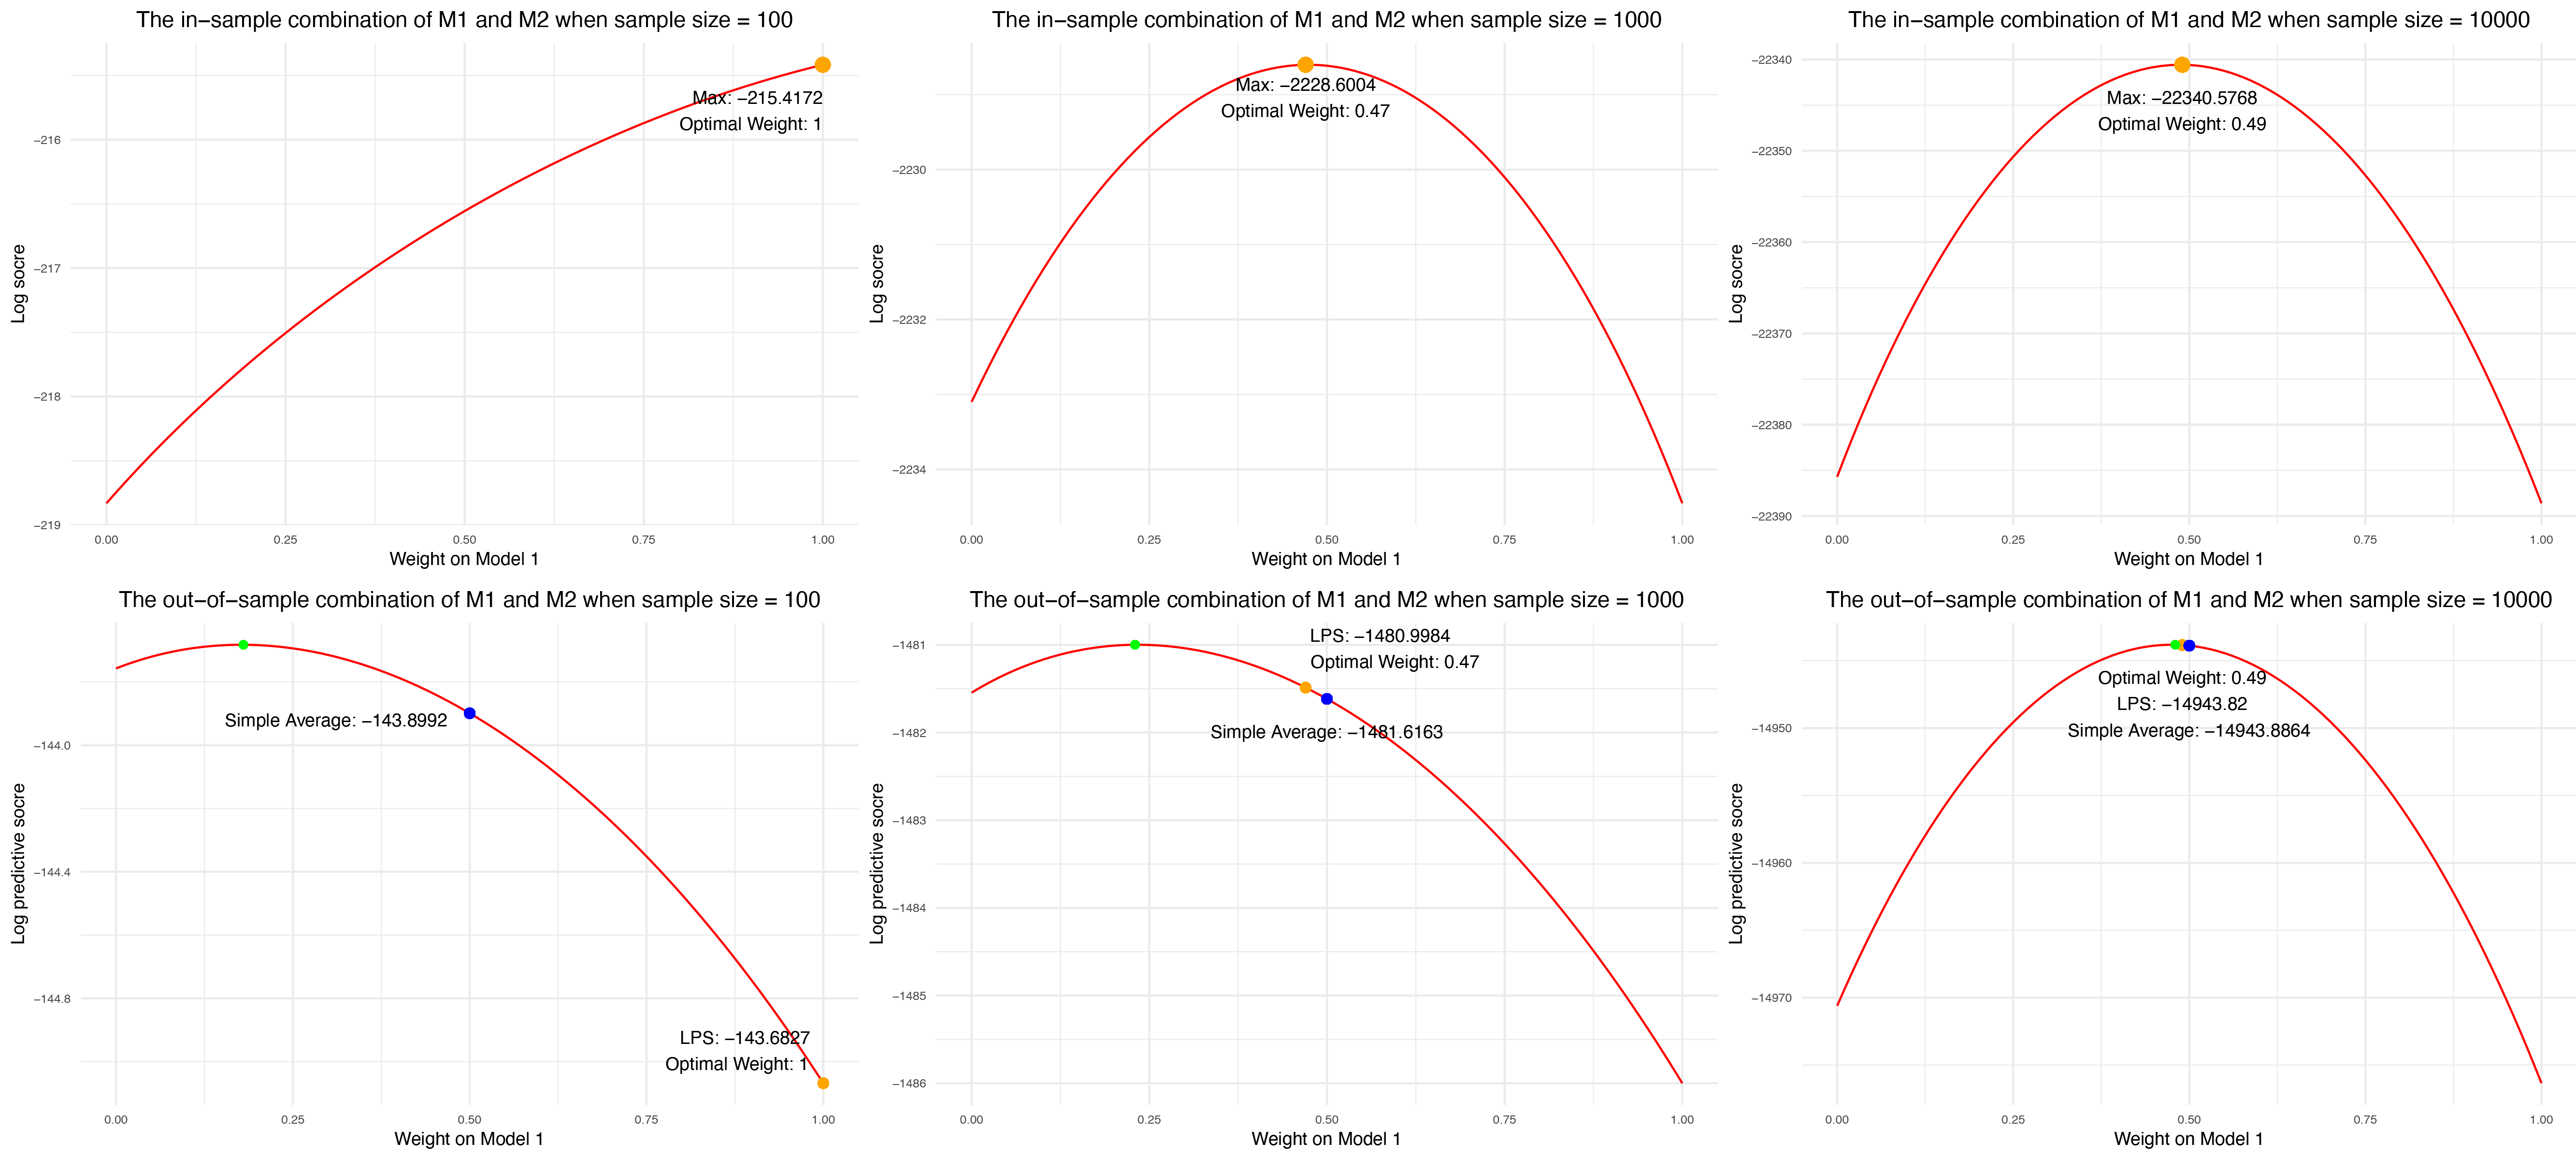
\includegraphics[scale=0.35]{figures/Sample_Size_100-10000.png}
\caption{Three columns refer to cases when $N=100$, $N=1000$, and $N=10000$ respectively while keeping all others constant as the initial set-up. The top graphs represent the in-sample combination performance and the bottom graphs represent the out-of-sample combination accuracy. The meanings of colored dots are the same as those in Figure \ref{fig:ss15000}.}
\label{fig:ss}
\end{figure}

First, it is notable that, in Figure \ref{fig:ss}, the performances of in-sample and out-of-sample combinations have completely different shapes or features when \(N=100\) but are gradually similar when \(N=1000\) and \(N=10000\). In the \(N=100\) case, we completely prefer Model 1 to fit the training set, however, the Model 1 becomes the worse choice for the test set. Thus, the averaged density forecast performs much better than the combination recommended by the optimal weight. This implies that the model combination which fits the in-sample well does not necessarily generate better forecasts when the sample size is small. Second, the forecast accuracy of optimal combination and that of simple averaging are getting closer when the sample size increases, which indicates the presence of the forecast combination puzzle. Roughly, the puzzle becomes noticeable when the sample size is larger than 500.

When we have a small dataset, it is not representative of the whole population, so the model estimation involves more randomness and is highly influenced by potential outliers. There is also a possibility of overfitting the training set when the training and test sets have distinct patterns. Therefore, given a large enough dataset and two equally good models, we are very likely to have the puzzle.

\begin{itemize}
\tightlist
\item
  \bf{Magnitude and Sign of $\pmb{\beta}$}
\end{itemize}

Next, the sample size is set to be 10000 so that it is large enough to reveal the puzzle. Consider the change in magnitude and sign of \(\beta_1\) and \(\beta_2\).

\begin{figure}[ht]
\centering
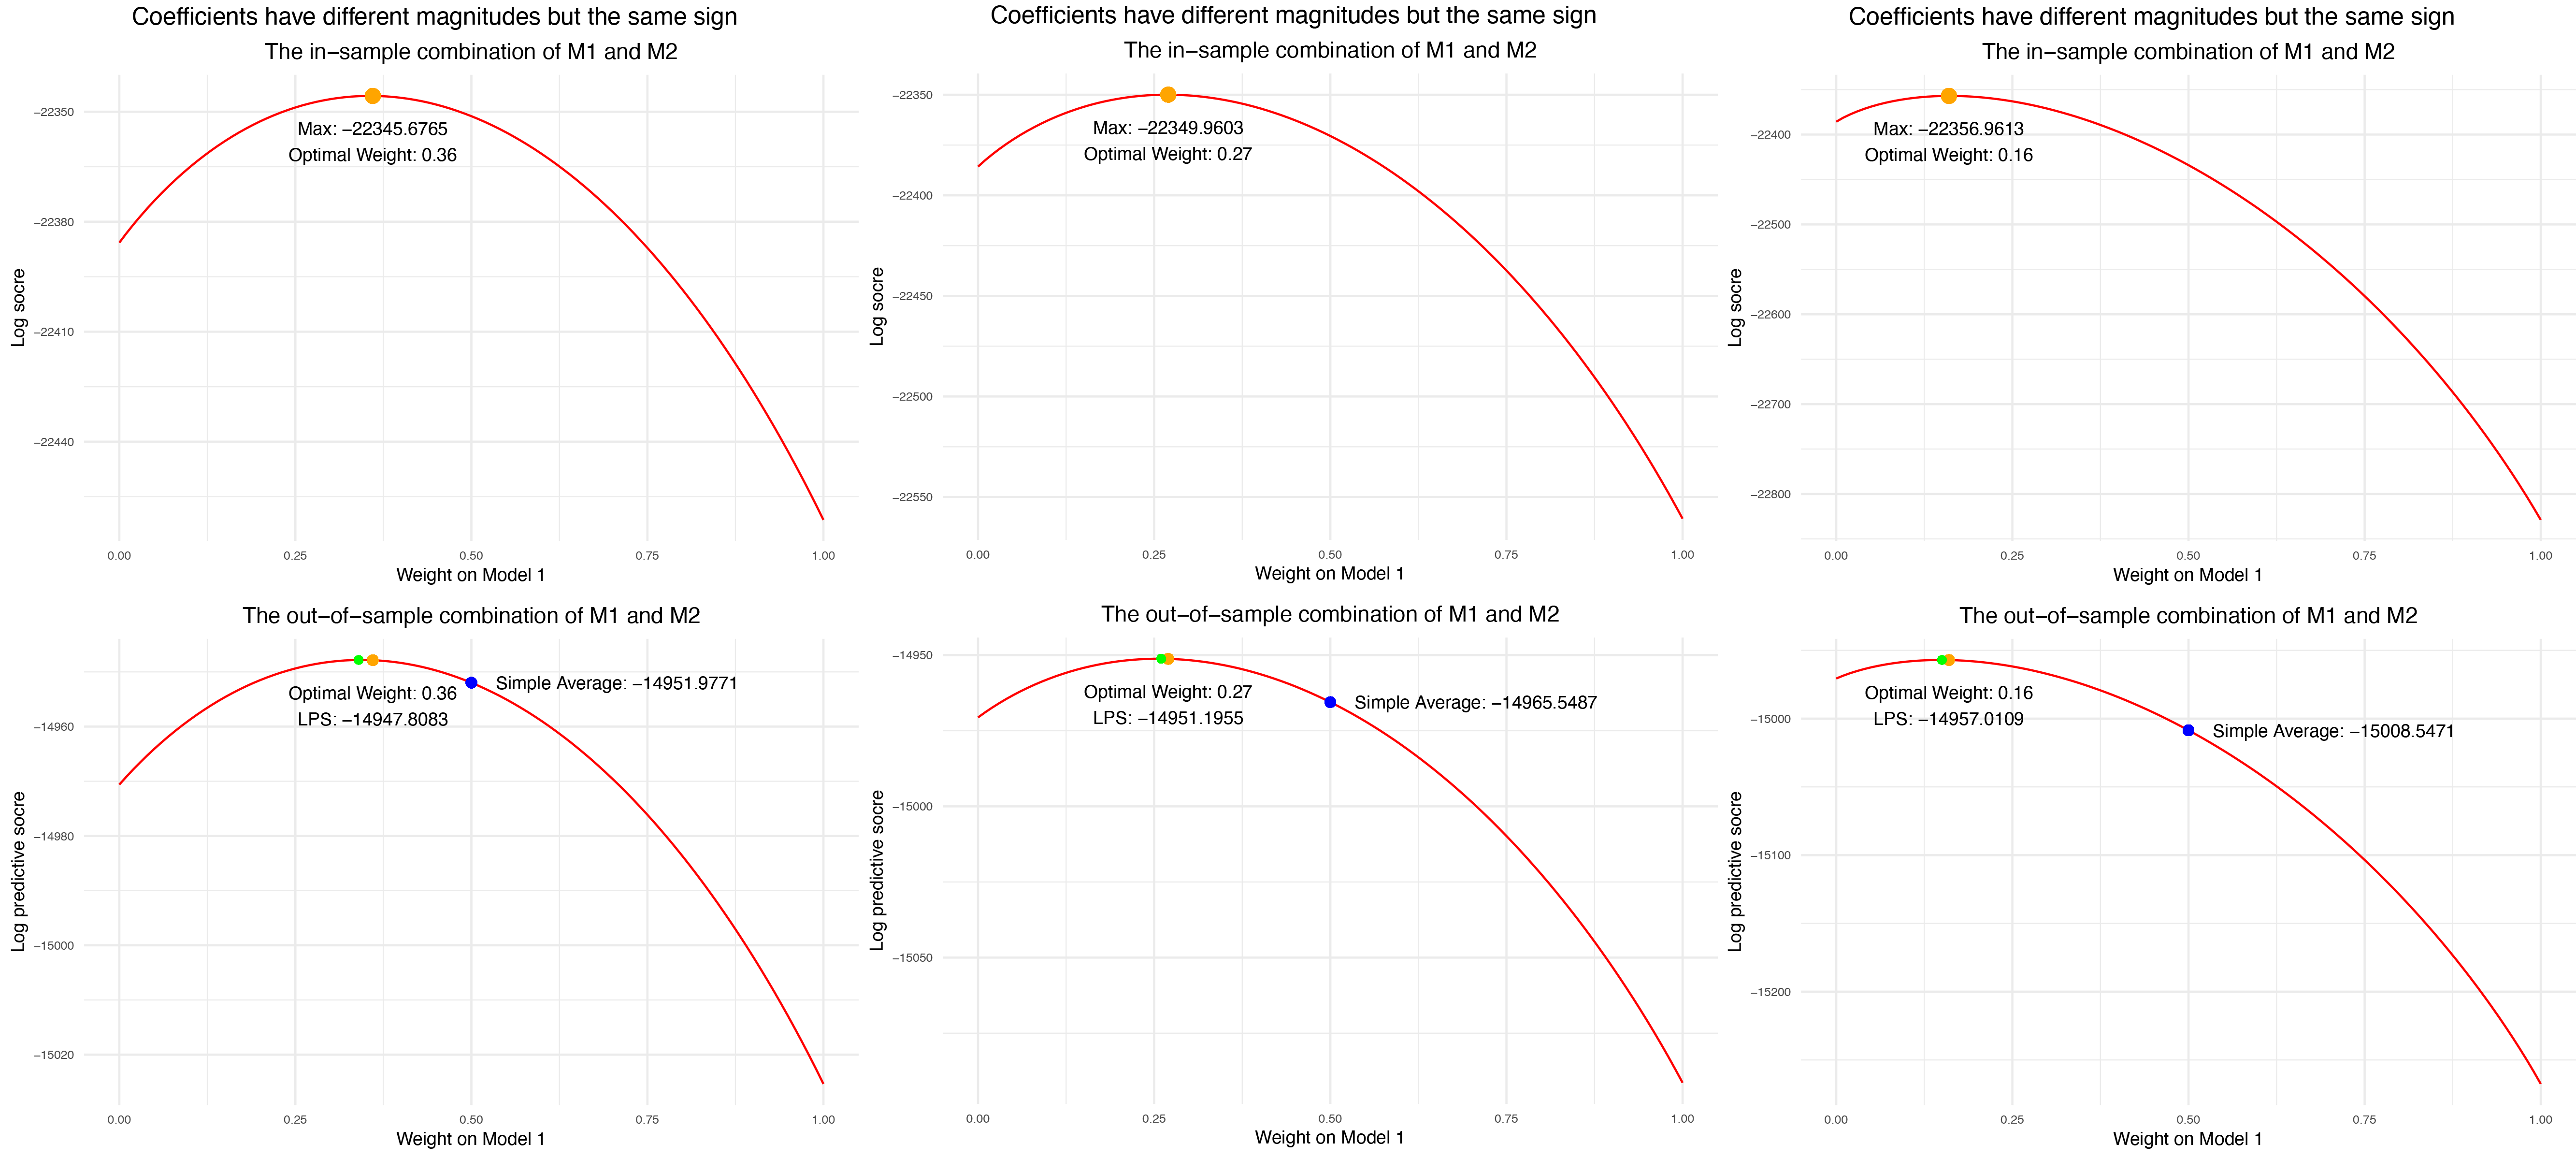
\includegraphics[scale=0.35]{figures/Beta_diff_mag.png}
\caption{In this case, $\beta_1$ and $\beta_2$ have the same sign but different magnitudes. The first column refers to $\beta_1=2$ and $\beta_2=3$, the second column refers to $\beta_1=2$ and $\beta_2=4$, and the first column refers to $\beta_1=2$ and $\beta_2=6$.}
\label{fig:magnitude}
\end{figure}

Based on the results shown in Figure \ref{fig:magnitude}, the puzzle is highly sensitive to the absolute difference between two parameters. If the absolute difference is large enough, generally more than half of the smaller coefficient, it is hard to observe the puzzle and the optimal combination always wins with a higher log predictive score. The larger the absolute difference, the bigger the difference of two log predictive scores.

In the linear regression analysis, the magnitude of each coefficient represents the influence size of each regressor on the dependent variable. A large coefficient means that a change in the corresponding regressor affects the dependent variable more in magnitude. Knowing this, it is reasonable to observe that the Model 1 has a decreasing weight in the optimal combination from left to right in Figure \ref{fig:magnitude}. The effect of \(x_2i\) on \(y_i\), \(\beta_2\), is relatively larger than the effect of \(x_1i\) on \(y_i\), \(\beta_1\), so the Model 2 with \(x_2i\) only should be weighted higher in the combination.

\begin{figure}[ht]
\centering
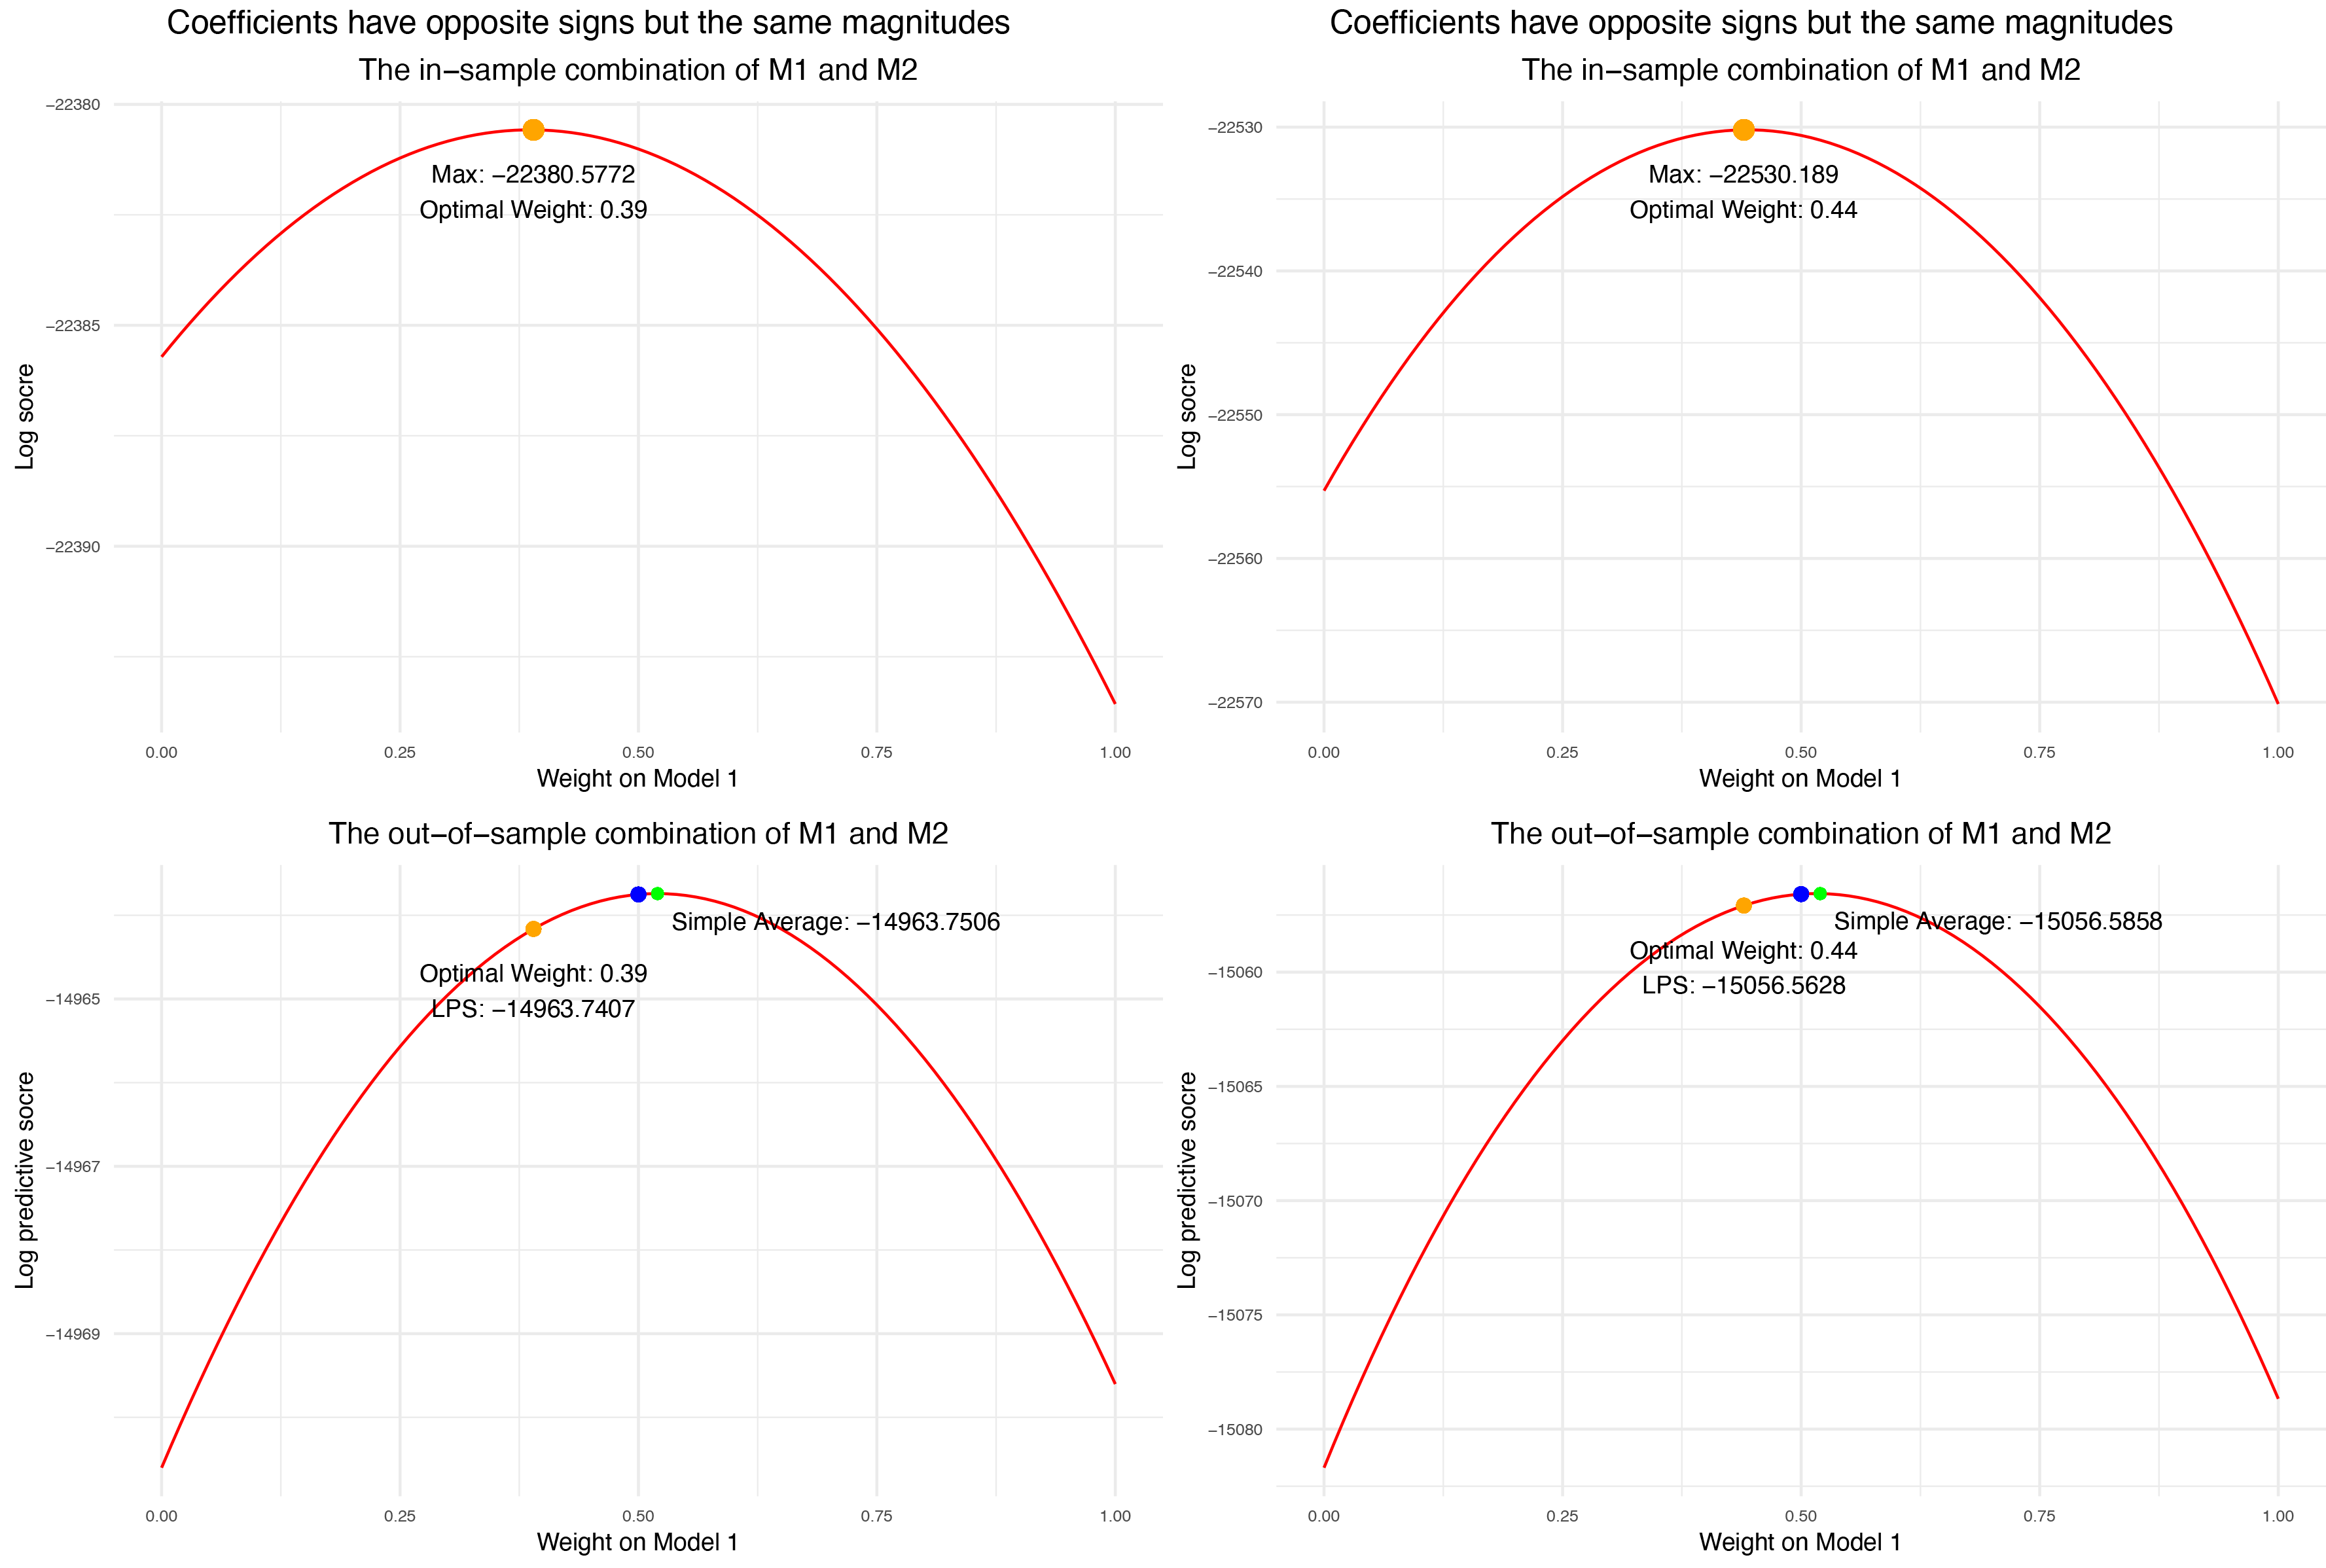
\includegraphics[scale=0.55]{figures/Beta_diff_sign.png}
\caption{$\beta_1$ and $\beta_2$ have the same magnitude but different signs, i.e. $\beta_1=-\beta_2$. The first column considers the case when $\beta_1=2$ and $\beta_2=-2$ and the second column considers the case when $\beta_1=4$ and $\beta_2=-4$.}
\label{fig:sign}
\end{figure}

Figure \ref{fig:magnitude} illustrate that when \(\beta_1\) and \(\beta_2\) only have opposite signs, the puzzle seems to be insensitive. In both cases, the optimal combination and simple averaging forecast have very similar log predictive scores, which is a strong evidence of the puzzle. Meanwhile, two regressors have the same effect in magnitude on \(y_i\), therefore, the weight should be equally assigned in rough. We also notice that the accuracy of the optimal prediction combination can be improved by having higher absolute values of the coefficients. This makes regressors to have larger and more certain impacts on \(y_i\), which is substantiated by the above case.

\begin{itemize}
\tightlist
\item
  \bf{Variance of regressors}
\end{itemize}

\begin{figure}[ht]
\centering
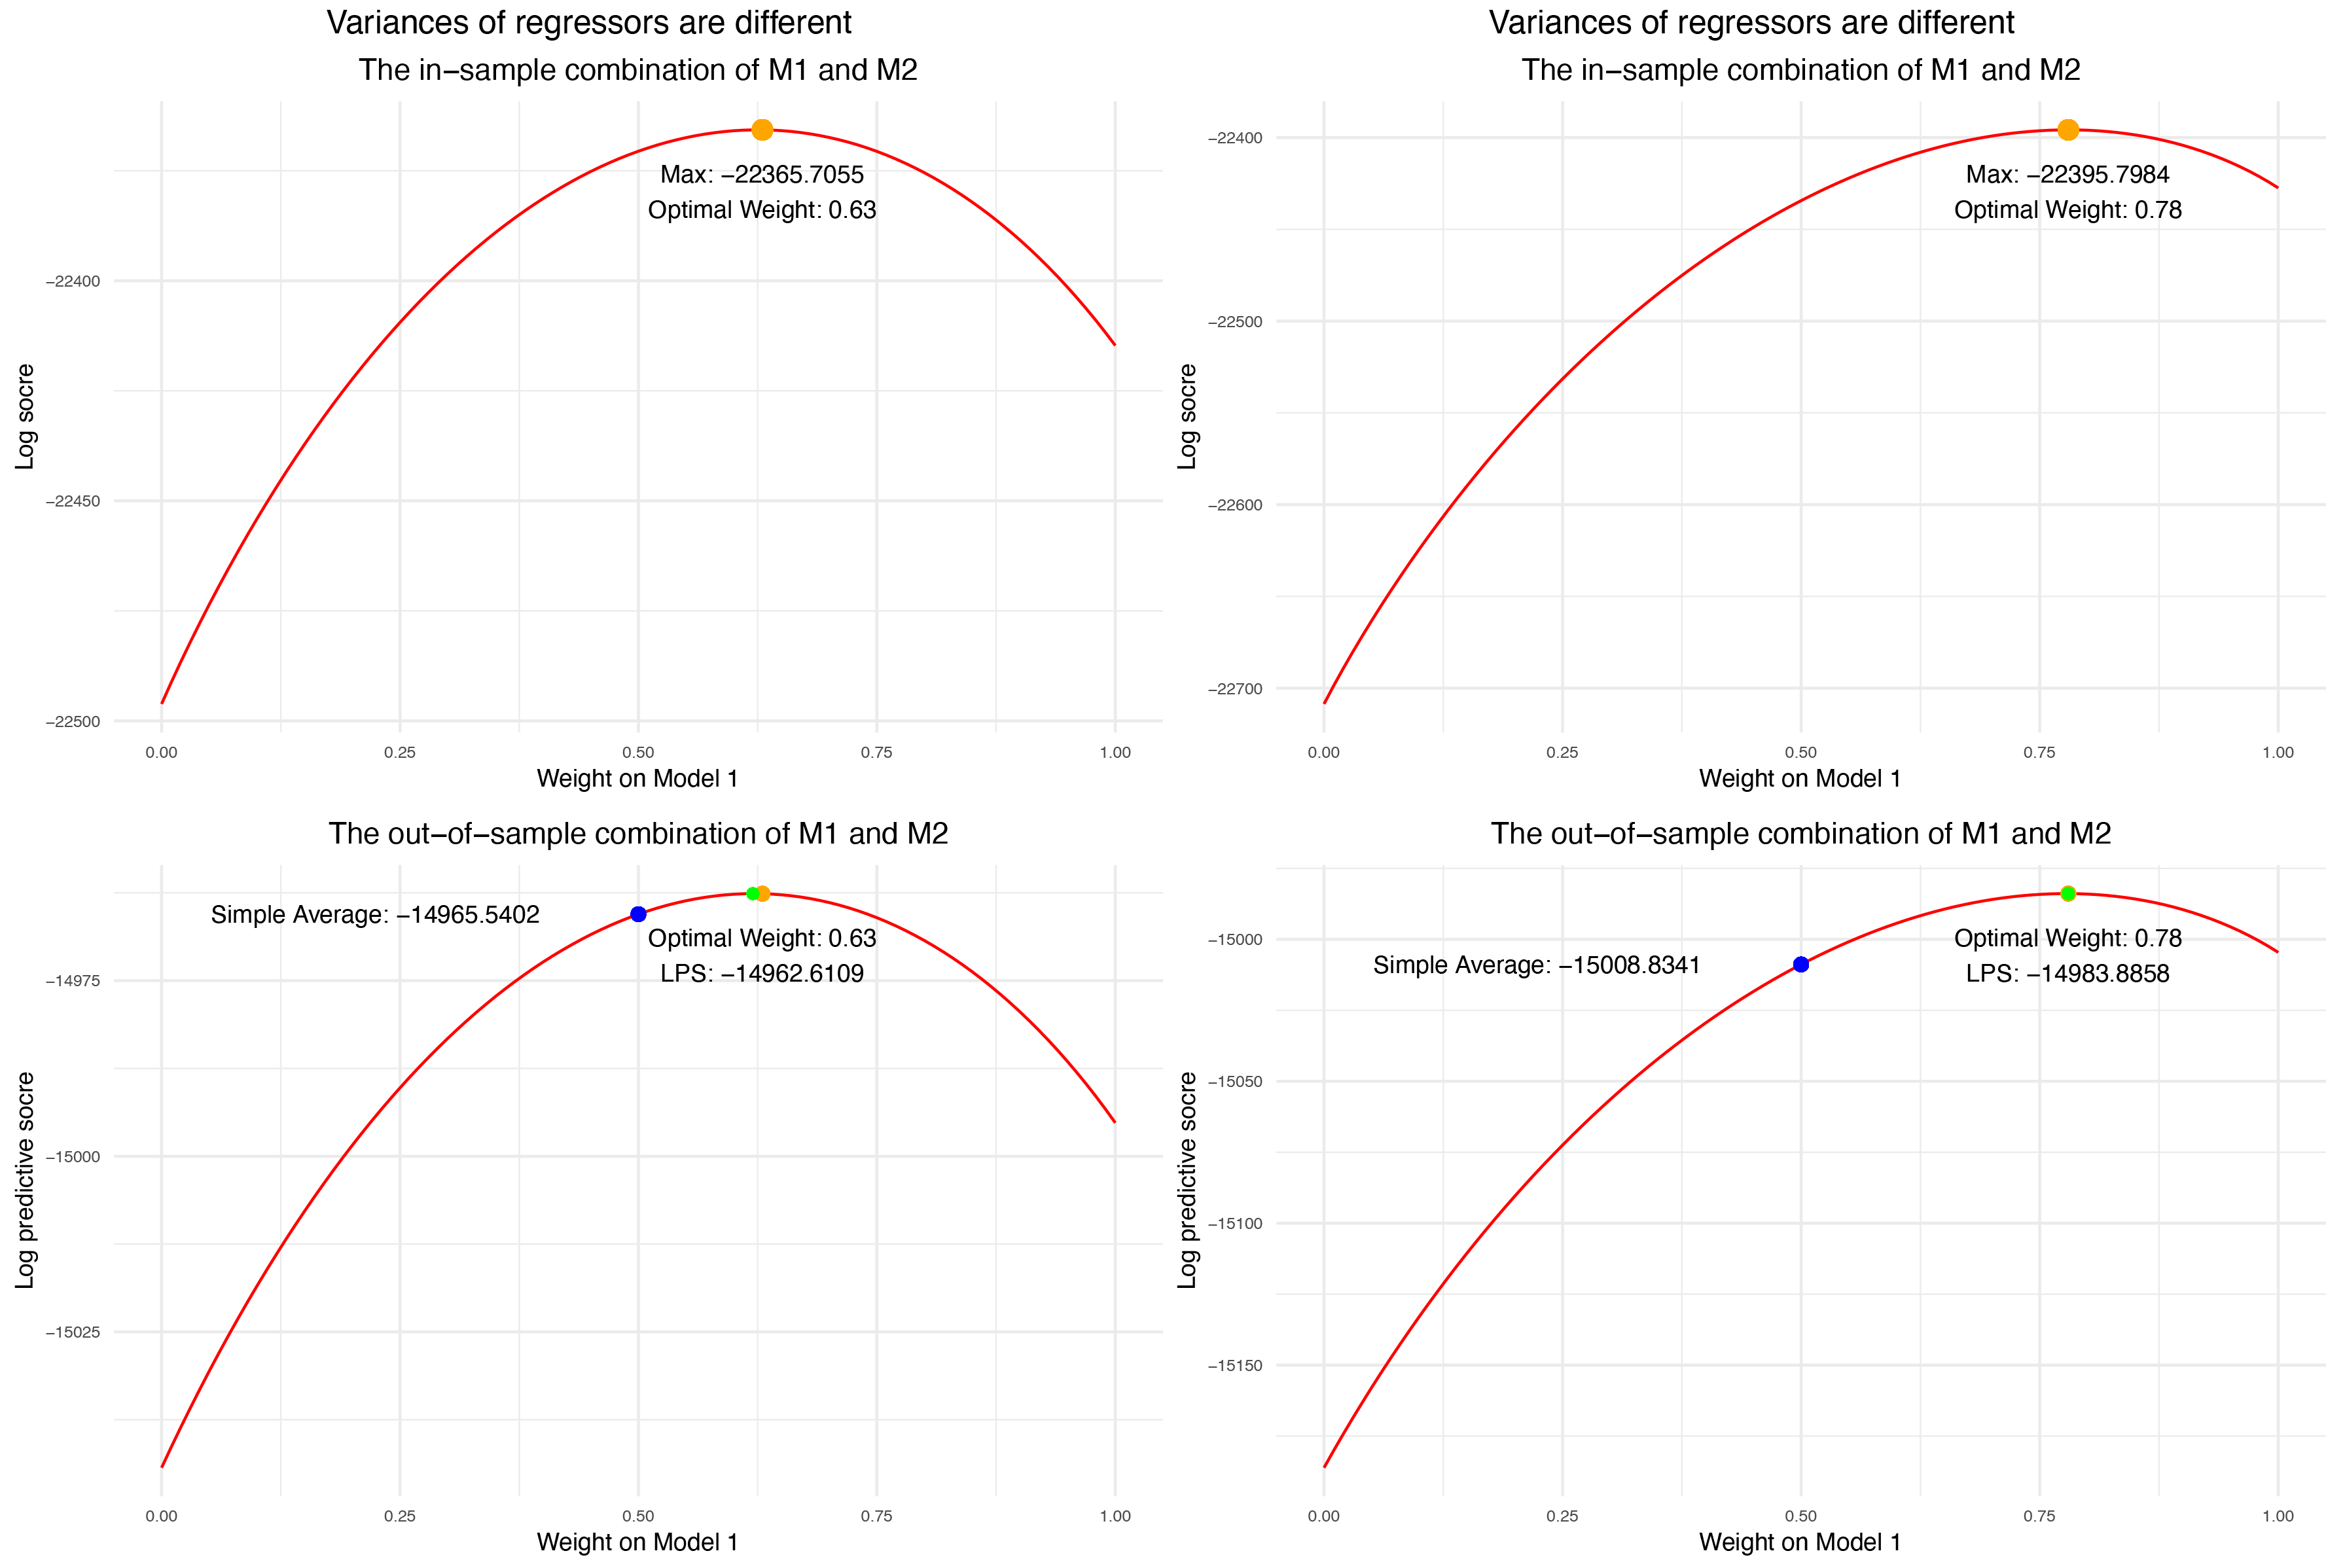
\includegraphics[scale=0.35]{figures/x_var.png}
\caption{The first column refers to the case when }
\label{fig:xvar}
\end{figure}

larger variance, more variation to explain y, more favored

Variance of the error term will influence the log score value
Pattern is hard to determine

\hypertarget{discussion}{%
\chapter{Discussion}\label{discussion}}

\hypertarget{research-objective-1}{%
\section{Research Objective}\label{research-objective-1}}

\hypertarget{conclusion}{%
\chapter{Conclusion}\label{conclusion}}

We focused on the combination of two individual forecasts for two reasons, which in most cases apply for the prediction of business figures in enterprises. Typically, a judgmental forecast and one that is derived using purely statistical means are available and corporate planning can be based on one of the forecast or a combination of both forecasts, where additional forecasts cannot be expected to introduce as much additional information. Furthermore, focusing on the two-forecast case allowed us to provide a variety of in-depth analyses. The challenge of extending the model and the decision boundaries to a larger, arbitrary number of forecasts is subject to future research.

This step, while important, is sizeable and we leave it to future work.

\appendix

\hypertarget{appendix}{%
\chapter{Appendix}\label{appendix}}

Exact formulas and explanations of these models can be found in \textcite{fpp3}. The formula of the conditional variance for the ETS models in this case is discussed in Chapter 6.3 of \textcite{HKOS08}. All codes are performed in R Statistical Software (version 4.2.1 (2022-06-23)). The packages used are \texttt{tidyverse} \autocite{tidy19}, \texttt{dplyr} \autocite{dplyr23}, and \texttt{fpp3} \autocite{fpp23}.

\printbibliography[title={Reference}]




\end{document}
